\section{Methods}

\subsection{Participants}
We first piloted the procedure and materials to identify potential issues with item wording or response options before preregistering. The pilot included 128 participants (68 women). Age was not collected as a continuous variable; instead, participants reported their age in categorical bands. The age distribution was as follows: 18-24 (\textit{N} = 25; 19.5\%), 25-34 (\textit{N} = 25; 19.5\%), 35-44 (\textit{N} = 20; 15.6\%), 45-54 (\textit{N} = 23; 18.0\%), 55-64 (\textit{N} = 17; 13.3\%), and 65+ (\textit{N} = 18; 14.1\%).

An \textit{a priori} power analysis using G*Power for a multiple regression (fixed model, test of a single regression coefficient) with 10 predictors indicated that a sample size of \textit{N} = 652 per country would provide 95\% power ($\alpha$ = .05, two-tailed) to detect a small effect of one predictor (\textit{$f^2$ = .02}). To ensure data quality, we used a 7-point satisficing scale (1 = strongly disagree, 7 = strongly agree; \citealp{berry2022drivers}). Participants answered six items assessing inattentive responding. Higher scores indicated greater satisficing, and participants with an average score of 4 or higher were excluded. Participants with a reCAPTCHA score of .50 or lower were classified as bots and excluded. We continued sampling until reaching 652 eligible participants per country, as specified in our preregistration. For the UK and US, samples were stratified to be broadly representative on age, gender, and race/ethnicity; for Denmark, quotas were applied on age and gender. Participants were at least 18 years old.

Before exclusions, we sampled 688, 876, and 714 participants from the UK, Denmark, and the US, respectively. We excluded 31, 164, and 42 participants as satisficers and 0, 55, and 19 participants as likely bots from the UK, Denmark, and the US, respectively. Final sample sizes were 657, 657, and 652 eligible participants recruited via Prolific (UK), Norstat (Denmark), and CloudResearch (US). The larger number of exclusions in the Danish sample may partly reflect differences in recruitment panels and upstream screening procedures. In the final samples, the British sample included \input{Results/Demographics_Results_UK/total_women} women (\textit{Mean}$_{\mathrm{age}}$ = 47.99, \textit{SD} = 15.00%
; \input{Results/Demographics_Results_UK/no_age} did not report age), the Danish sample included \input{Results/Demographics_Results_DK/total_women} women and \input{Results/Demographics_Results_DK/total_non_binary} nonbinary individuals (\textit{Mean}$_{\mathrm{age}}$ = 50.26, \textit{SD} = 16.68%
; \input{Results/Demographics_Results_DK/no_age} did not report age), and the American sample included \input{Results/Demographics_Results_US/total_women} women (\textit{Mean}$_{\mathrm{age}}$ = 46.17, \textit{SD} = 14.70%
; \input{Results/Demographics_Results_US/no_age} did not report age). 
The Danish sample had the highest knowledge (\textit{Mean} = 3.44, \textit{SD} = 1.31%
) and familiarity (\textit{Mean} = 4.09, \textit{SD} = 1.39%
), followed by the US (\textit{Mean} = 2.77, \textit{SD} = 1.46%
; 
\textit{Mean} = 3.10, \textit{SD} = 1.54%
), and, lastly, the UK (\textit{Mean} = 2.23, \textit{SD} = 1.31%
; \textit{Mean} = 2.33, \textit{SD} = 1.34%
). The study protocol received approval from an institutional ethics review committee, and all participants provided informed consent. All participants received compensation equivalent to €4 in their local currency for completing the 25-minute questionnaire.

\subsection{Procedure}
The survey consisted of five stages (Figure \ref{fig:procedure}).

\subsubsection{Stage 1: Introduction to Endocrine-Disrupting Chemicals}

Participants received a brief introduction to EDCs, including examples such as pesticides in produce and bisphenol A in plastics (Figure \ref{fig:comprehension_check}). They were then asked to identify five EDCs from a randomized list of ten compounds and materials based on the information just presented. Participants could proceed only after correctly selecting the five EDCs. Selecting all options was not possible. If participants failed to identify all EDCs, they received a short reminder describing EDCs and their common sources.

\begin{figure}[t]
    \centering
    \caption{\textbf{Participant Comprehension Check for Different EDCs Mentioned in the Study}}
    
\includegraphics[width=\linewidth]{Additional_materials/combined_figure_abc_horizontal.png}
    \caption*{Before starting the survey, participants first completed a comprehension check. \textbf{a.} Participants were first given the definition of EDCs within the context of the survey. \textbf{b.} Participants were then given information on where certain EDCs can be found in everyday life (e.g., bisphenol A in some plastics). \textbf{c.} Example of verbatim sentences participants were shown.}
    \label{fig:comprehension_check}
\end{figure}

\subsubsection{Stage 2: Risk Attributes}

Participants rated 18 exposure scenarios on nine risk attributes identified in prior research \citep{fischhoff1978safe}. The 18 exposure scenarios were selected to represent three common exposure pathways: consumption, inhalation, and dermal application, while including the same EDC categories across pathways. Candidate chemical classes and exposure scenarios were informed by the Endocrine Society’s overview \citep{endocrinesociety_common_edcs_nd} of commonly discussed EDCs and their occurrence in everyday life. We selected 18 exposure scenarios to provide broad coverage across exposure pathways while maintaining a feasible survey length and minimizing fatigue effects.
The selection of chemical categories was guided by a systematic literature review of factors influencing perceived health risks of EDCs \citep{pravednikov2024main}. We selected six commonly discussed EDC-related chemical categories that could be embedded in comparable everyday exposure scenarios across the three exposure pathways.
Scenarios were described using a combination of broader chemical categories and specific chemical labels to balance scientific precision with recognizability across countries.

The nine attributes included voluntariness of risk, immediacy of effect, knowledge about the risk for exposed individuals, knowledge about the risk within the scientific community, control over the risk, newness, chronic versus catastrophic impact, common versus dread risk, and severity of consequences.

All activities were rated on 7-point scales. The order of activities within each attribute was randomized, but the order of attributes was fixed. Examples included drinking water from plastic bottles containing bisphenol A (BPA), applying sunscreen containing parabens, and breathing air containing phthalates from indoor air fresheners. The full list of exposure scenarios and the attribute order are provided in Supplementary Section S1.

\subsubsection{Stage 3: Pathway-Specific Ranking of Perceived Health Risk}

%Participants evaluated the perceived severity of health risks associated with the same 18 EDC-related activities described earlier.
Participants evaluated the perceived health risks associated with the same 18 EDC-related scenarios described earlier. Because our research question concerned the relative prioritization of perceived health risks across exposure scenarios, we used a forced-ranking procedure rather than independent Likert-scale ratings. This procedure allowed participants to directly compare scenarios against one another, making the ratings relative judgments across scenarios rather than independent evaluations of each activity in isolation.
Participants first saw the full list and ranked the six activities they believed posed the highest health risk (1 = highest risk, 6 = lowest risk). After submitting their rankings, those activities were removed and the next 6 activities were presented again for ranking. This procedure was repeated until all 18 activities were ranked. The order of activities was randomized at each step. Participants ranked only six activities at a time to reduce cognitive load.

Because higher rank numbers represented lower perceived risk, greater mean values indicate lower perceived health risk. Although participants ranked activities in three separate blocks, we created a sequential ranking distance variable by numbering ranks from 1 to 18 across blocks. For example, ratings in the first block were coded 1-6, ratings in the second block 7-12, and ratings in the third block 13-18. This allowed us to analyze the rankings as a single ordered sequence.

\subsubsection{Stage 4: Health Beliefs}

Participants reported how likely they believed they were to become ill from EDCs in the next twelve months (perceived susceptibility), how serious they believed such illness would be (perceived severity), and how large they perceived the general health risks of EDCs to be (perceived overall health risk). All three health belief measures were assessed on 7-point Likert scales, with endpoints ranging from \textit{Very unlikely} to \textit{Very likely}. Exact wording is provided in Supplementary Section S2.

\subsubsection{Stage 5: Trust, Knowledge, and Demographics}

Participants rated their trust in institutions using six items (e.g., “I believe that scientists have the capability to accurately assess the risks associated with endocrine-disrupting chemicals”). Trust was measured on 7-point Likert scales ranging from \textit{Strongly disagree} to \textit{Strongly agree}. Subjective knowledge and familiarity (before participating in the study) with EDCs were assessed on separate 7-point scales, with endpoints ranging from \textit{Very little} to \textit{Very much} (knowledge) and from \textit{Not familiar at all} to \textit{Very familiar} (familiarity) (see Supplementary S3). They then provided demographic information, including age, education, employment, geographical residence, household income, number of children in the household, and perceived health. We included these variables as regression predictors because prior research identifies them as correlates of EDC risk perceptions \citep{pravednikov2024main}. The satisficing questionnaire \citep{berry2022drivers} was administered between the trust items and the demographic questions.

\begin{figure}[t]
    \centering
    \caption{\textbf{Overview of the Five-Stage Survey Design}}
    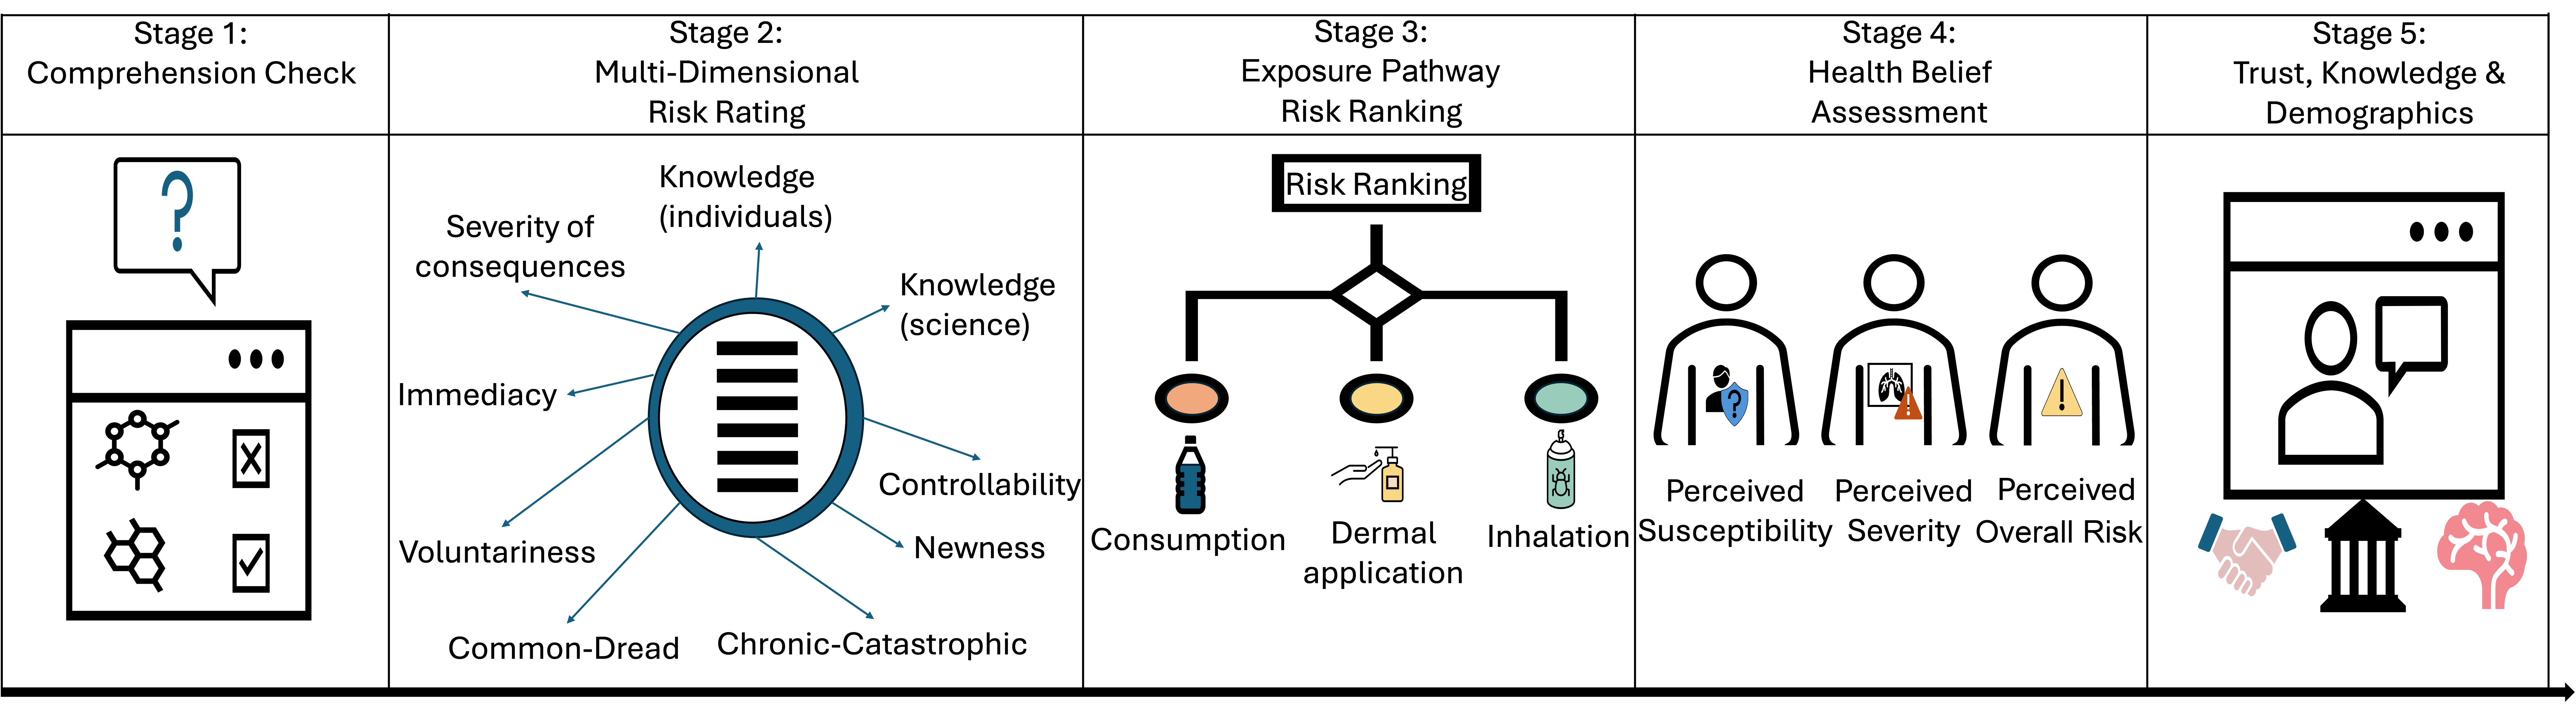
\includegraphics[width=\linewidth]{Additional_materials/procedure.png}
    \caption*{The survey procedure consisted of five distinct stages designed to map risk perceptions of endocrine-disrupting chemicals (EDCs). Stage 1 served as an informational primer and comprehension check where participants had to correctly identify five EDCs from a list of ten compounds to proceed. In Stage 2, participants provided multi-dimensional risk ratings for 18 exposure scenarios across nine canonical risk attributes. Stage 3 involved an exposure pathway risk ranking, where participants ranked the same 18 activities to identify which of the primary pathways -- consumption, dermal application, or inhalation -- they perceived as most hazardous. Stage 4 measured three core health beliefs: perceived susceptibility (likelihood of illness), perceived severity (seriousness of illness), and general perceived overall health risk. Finally, Stage 5 collected data on institutional trust, subjective knowledge, and a set of sociodemographic variables.}
    \label{fig:procedure}
\end{figure}

\subsection{Statistical Analyses}
To examine how participants perceived EDC risks across the nine risk attributes identified in prior research \citep{fischhoff1978safe}, we conducted a principal component analysis (PCA) with varimax rotation. The number of components was determined using the Kaiser criterion (i.e., retaining components with Eigenvalues > 1). Sampling adequacy was evaluated using the Kaiser-Meyer-Olkin (KMO) statistic, and Bartlett's test of sphericity was used to verify that the correlation matrix was suitable for dimension reduction. We hypothesized that EDC risks would generally be perceived as involuntary, delayed, not well-known to the general public, well-known to scientists, controllable, new (except pesticides), neither chronic nor catastrophic, neither common nor dreaded, and not necessarily fatal.

We further expected that risk perception would vary by type of activity involving exposure to EDCs. Specifically, we predicted that activities involving ingestion (e.g., food or water) would be perceived as riskier than those involving dermal exposure, and that dermal exposure would be perceived as riskier than inhalation. To test these hypotheses, we conducted a one-way analysis of variance (ANOVA). Assumptions were examined prior to fitting the model, including homogeneity of variance using Levene's test. When the homogeneity assumption was violated, we used the nonparametric Kruskal-Wallis rank-sum test in place of the one-way ANOVA. Statistically significant omnibus effects were followed by appropriate post hoc comparisons with adjusted \textit{p}-values.

Finally, multiple regression analyses were used to examine which sociodemographic and psychological factors predicted three perceived EDC health beliefs: perceived severity, perceived susceptibility, and perceived overall health risk. Predictor variables included institutional trust, knowledge about EDCs, familiarity with EDCs, age, gender, educational level, employment status, geographical residence, annual household income, number of children in the household, and perceived health. Number of children was recoded into a binary variable (children present vs. none). Prior to estimation, model assumptions were assessed using the Ramsey RESET test (nonlinearity), variance inflation factors (multicollinearity), the Breusch-Pagan test (heteroscedasticity), the Shapiro-Wilk test and Q-Q plots (normality), and the Durbin-Watson statistic (autocorrelation).

Data pre-processing was conducted in Python v3.12.0 \citep{python} using primarily the Pandas library \citep{pandas}, and all statistical analyses were conducted in R v4.3.1 \citep{rRef}. The study was preregistered (https://osf.io/yds73/), and unless otherwise noted, analyses followed the preregistered plan. Qualtrics survey files, analysis scripts, and processed data are available at https://github.com/Nick-Simonsen/EDC\_risk\_perception.
